\section{Self Power Modeling Methodology}
\label{sec:method}

In this section, we describe the basic self power modeling methodology,
we added the constraints to the basic solver in an effort to help the solver to output meaningful model parameters, and for the usabiity of Android phones power sensor readings.  

% as depicted in Figure~\ref{fig:equations}.
\if 0
\begin{figure}[tp]
    \centering
    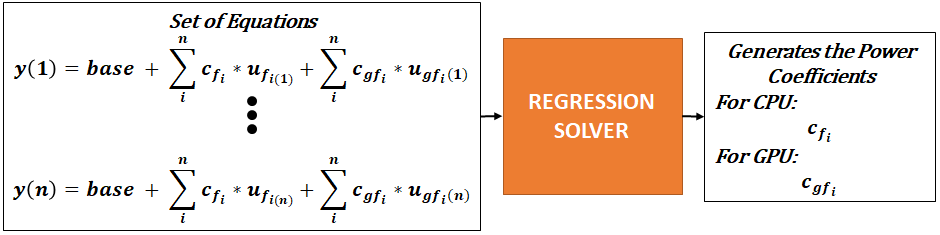
\includegraphics[width=0.95\columnwidth]{figures/design_2.png}
    \vspace{-0.1in}
    \caption{SPMD via solving a system of linear equations.}
    \label{fig:equations}
    \vspace{-0.1in}
\end{figure}
\fi

\begin{table}[t]
{\footnotesize
    \centering
    \caption{Power state, utilization, and energy collected during online app run.}
    \vspace{-0.1in}
   % \begin{tabular}{|p{32mm}|p{10mm}|p{23mm}|}
    \begin{tabular}{|l|P{11mm}|c|}
    \hline
          &  Symbol & Collection method \\
         \hline
         \multicolumn{1}{|l|}{\textbf{Power State}} &  &   \\
         CPU Frequency      & $f_{k}$                               & cpu\_frequency \\
         GPU Frequency      & $g_{k}$                               & kgsl\_pwrlevel \\
         GPU State          & $s_j$                                 & kgsl\_pwr\_set\_state \\
         \hline
          \multicolumn{1}{|l|}{\textbf{Utilization}} &   &  \\
         
         \multicolumn{1}{|l|}{CPU Util. in freq. $f_k$}               & $u^c(f_{k})$        & cpu\_idle \\
         \multicolumn{1}{|l|}{GPU Util. in freq. $g_k$, state $s_j$}  & $u^g(g_k,s_j)$      & kgsl\_pwrstats \\
         \hline
         \multicolumn{1}{|l|}{Energy drain}     & $y$                                &
         \multicolumn{1}{p{30mm}|}{/sys/class/power\_supply /charge\_counter} \\
         \hline
    \end{tabular}
    \label{tab:triggers}
    \vspace{-0.1in}
}
\end{table}


% \comment{Placeholder: We may or may not need to discuss power triggers for other phone components
% to make this section general.}

\subsection{Basic SPMD Process}
\label{subsec:generic}

As discussed in \S\ref{subsec:spmd}, SPMD consists of two basic steps: 
online data collection for setting up a system of equations and 
offline model derivation by solving the system of equations.

\paragraph{Online data collection}
Since SPMD is "in-situ", collecting data  is needed to set up the equations  while the app is running. 
% As discussed in \S\ref{sec:primer}, in modern phones, the CPU and GPU power draw are 
% functions of the operating frequency and the power state (for GPU). Therefore,
% for power triggers, we need to collect the duration each component spends in every 
% combination of frequency and power-state during the app run, as listed in Table~\ref{tab:triggers}.
%
Table~\ref{tab:triggers} lists the data that need to be collected and how they are collected. 
The data include the power states and utilization in each state , for each component used by the app  , for each time interval corresponding to an equation as well as  the whole-phone energy drain.

We use the Linux event trace~\cite{eventtrace} to collect the power state and utilization. 
To collect whole-phone energy draw per interval, we can use either the built-in power sensor energy counter which became available since Android \comment{7}, or an external power monitor such as Monsoon~\cite{monsoonpowermonitor}.

\cut{ Ideally, reading from the built-in power sensor is preferred, since it does not require wiring the phone battery and potentially allows SPMD to be performed on any phones, including users' phones "in the wild". However, as we will see in the next section, built-in power sensor readings have such high error that makes them impractical to use in SPMD. 
}

\if 0
\begin{figure}[tp]
{\small
    \centering
    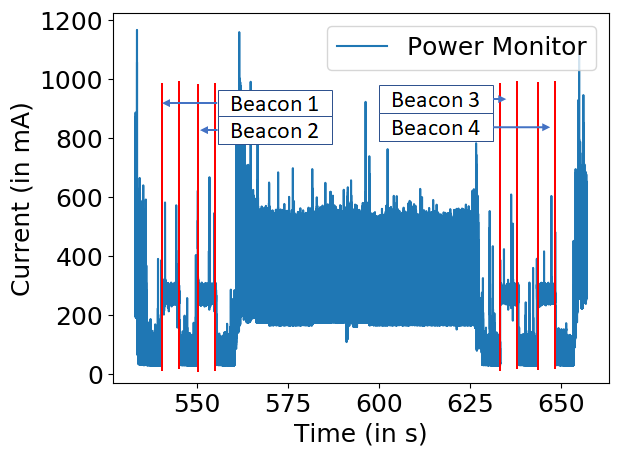
\includegraphics[width=0.80\columnwidth]{figures/beacons_3.png}
    \vspace{-0.1in}
    \caption{Beacons to align power monitor with phone clock.}
    \label{fig:align_beacon}
    \vspace{-0.1in}
}
\end{figure}
\fi

%%%%%%%%%%%%%%%
\paragraph{Offline model derivation} 
%
In offline processing, \eg when the app completes it running and data for model derivation is available, SPMD sets up a system of linear equations with the phone component power parameters as unknowns.
In general, the trace duration is cut into $K$ equal intervals of $T$ seconds each, and one equation is created for interval $t$ as follows:
\begin{equation}
y_t = p^{c}_{base}+ \sum_i\sum_k{u^c_t(f_k)*p_i^{c}(f_{k})} + 
            \sum_{j}\sum_{k} u^g_t(g_k,s_j)*p^{g}(g_k, s_j)
\end{equation}
where the double summation for the CPU is over all the CPU cores and frequencies,
the double summation for the GPU is over all the GPU frequencies and GPU states,
$u^c_t(f_k)$ and $u^g_t(g_k,s_j)$ are the CPU and GPU utilization for the corresponding power states
in time interval $k$,
and the left-hand-side (LHS) $y_t$ is the total phone energy drain in time interval $t$.
% where model parameter $p^c(f_{i})$ is the CPU power draw for frequency $f_i$,  
% model parameter $p^g_{ij}$ is the GPU power draw at frequency $f_i$ and power state $j$, the utilization coefficients $_{f_{i}}(k)$ and $u_{ij}(k)$ equal the total utilization (in seconds) of CPU and GPU in the corresponding frequencies and power states in the $k$th trace interval, and $y(k)$ denotes the total phone energy drain during interval $k$ from integrating power sensor or power monitor readings.
\cut{ 
Clearly, in a given app run, the CPU and GPU may not go through all possible frequencies and power states, and hence not all power parameters may show up in the equations. SPMD will only derive those power model
parameters actually encountered in the app run. This is not an issue with SPMD as only those parameters will be needed for the power model applications such as energy profiling or energy debugging. 
}

Since there can be more equations than the number of unknowns, 
the sytem of equations can be solved using a regression-based solver to generate the power parameters.
In this paper, we use the python curve\_fit() function which uses a non-linear least square fitting as our regression solver~\cite{curvefit}.

SPMD via solving a system of equations using a regression solver is conceptually simple. 
However in practice, the single biggest challenge is whether the system of equations 
has got enough diversity so that the regression solver
can generate meaningful solutions to the system of euations , \ie power model parameters. 

\if 0
\subsection{SPMD Challenges}
\label{subsec:challenges}

SPMD via solving a system of equations using a regression solver is conceptually simple. 
In practice, the single biggest challenge is whether the system of equations 
has enough diversity so that the regression solver
can generate meaningful solutions to the system, \ie power model parameters. 
The answer is not obvious for at least two reasons. 

{\bf Condition 1: Usage coefficients lack diversity.}
First, \S\ref{sec:primer} has concluded that
we need to set up a system of equations for each app scenario as different scenarios
even of the same app can have different component usage. However, 
one can imagine that the app behavior for the same app scenario may be highly repetitive and hence
the resulting equations, either the usage terms on one side or the energy drain on the other side,
 may look similar or only differ slightly, resulting on low rank of the equations. 

{\bf Condition 2:s Noisy energy measurement.}
The energy measurement can contain noise and if the difference among the true energy values for different equations is small, the noise level may dominate the energy variations of the different equations. This can result in the regression solver trying to minimize the fitting error from noisy energy measurement as opposed to fitting the true energy difference.  

Our verification study centers around addressing this challenge, by systematically exploring different ways of setting the system of equations to try to increase the diversity.

Before presenting our verification study, we discuss two refinements we added
to the basic SPMD methodology.


\fi

\subsection{Adding Constraints to the Solver}
\label{subsec:constraint}

\if 0 
As we will see in \S\ref{sec:modelling_macro}, 
when the system of liner equations suffers the two conditions above, the regression solver may output different solutions that all minimize the fitting error, which may violate basic properties of the power model parameter values. To overcome this, in addition to the basic unconstrained solver, 
\fi 
We experimented with adopting two ways for constraining the solutions generated by the regression solver based on simple domain knowledge, as shown in Table~\ref{tab:constrained}.

\begin{table}[tp]
%\questionaj{These constraints must also constrain GPU busy and idle.}
{\small
    \centering
    \caption{Constraints added to the regression solver.}
    \vspace{-0.1in}
    \begin{tabular}{|p{25mm}|p{52mm}|}
    \hline
         Constrainted SPMD  & \multicolumn{1}{c|}{Description} \\
         \hline
         Unconstrained      & No constraints are applied. \\
         Constrained        & Model parameters should not decrease with increasing frequencies. GPU idle power is less than Budy power. \\
         Freq-constrained   & CPU model parameters are modeled as a polynomial of frequency. \\
         \hline
    \end{tabular}
    \label{tab:constrained}
    \vspace{-0.1in}
}
\end{table}


\paragraph{Constraint 1: positivity and monotonicity}
Without any constraint, we found the regression solver can output CPU/GPU power values those are negative or 
decreasing while the frequency increases.
To prevent the solver from outputing such solutions, we add three constraints to the regression solver: 
(1) all model parameters should be positive;
(2) the model parameters with increasing frequencies for each component should be non-decreasing;
(3) the GPU Idle power should be lower than the GPU Busy power. 
We denote this version of SPMD as "Constrained SPMD" in Table~\ref{tab:constrained}.


\paragraph{Constraint 2: modeling CPU power as a function of frequency}
We found even with Constraint 1, the 
CPU power parameters output by the solver often does not change with varying frequencies. 
To make the CPU model parameters output more consistent with the reality, 
we exploited another domain knowledge about the CPU power draw,
that the power draw increases as per a low-order polynomial of the operating frequency~\cite{armdvfs,rizvandi2011some}.
% Since the specific polynomial function may vary for different phones, \eg early phones only performed % frequency scaling (FS) while newer phones perform dynamic voltage and frequency scaling (DVFS), we first used a simple CPU benchmark to find the order of the polynomial for each phone used in our experiments. 
%
\if 0
\begin{figure}[tp]
    \centering
%    \vspace{-0.1in}
    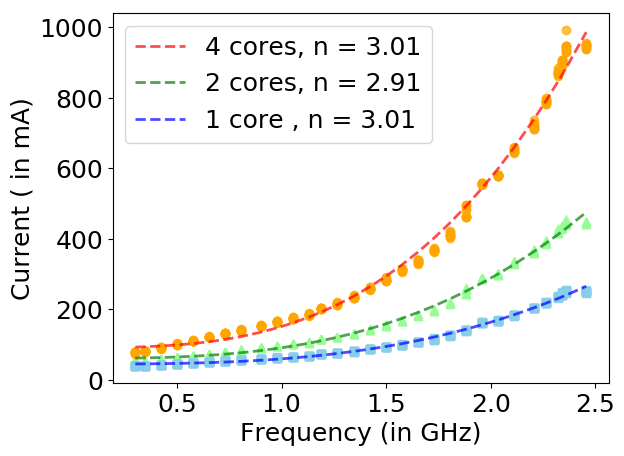
\includegraphics[width=0.80\columnwidth]{figures/cpu_characteristics.png}
    \caption{Moto Z3 big core CPU power draw grows with frequency 
    when running the arithmetic-intensive benchmark.}
    \label{fig:cpu_characteristic}
    \vspace{-0.1in}
\end{figure}
\fi
%
\cut{ We ran a microbenchmark that performs arithmetic-intensive or memory-intensive operations for 7 seconds
on 1, 2 and 4 big cores, for each big core frequency, and fit the measured phone power 
with a polynomial function in frequency.
%\begin{equation}
%     P_{CPU} = p^c_{base}+ \sum_i p^c_i({f_k}) = p_{base}+\sum_i  a*f_k^{n}
% \end{equation}
% Figure~\ref{fig:cpu_characteristic} shows the measured power draw and curve fitting on Moto Z3.
}
Our CPU microbenchmark results show show that 
% the fitted exponent $n$ for 1, 2 and 4 cores are 3.01, 2.97 and 3.01, respectively.
the per core power of Moto Z3 grows as the third-power of the CPU frequency.
Thus we replace all the CPU power parameters with third-power of the CPU frequency in the SPMD model equations.
%model the Moto Z3 big core power as a third-order polynomial of the CPU frequency in the model equations of SPMD.
%
Doing so has two benefits: (1) it reduces the number of CPU power parameters from $K$ - the number of CPU frequencies - to 2, $p_{base}$ and coefficient $a$, which reduces the number of equations needed for the solver; (2) it puts constraints for the CPU power  to be not only  monotonic, but consistent with physics.


\subsection{Can Power Sensor Readings be Used?}
\label{subsec:modelling_sensor}

Since using the built-in power sensor readings would allow SPMD to be performed on any phone in the wild,
we assess the feasibility of using the power sensors in modern smartphones for developing SPMD,
by measuring the accuracy of their the energy counter readings.

%{\bf Methodology }
%% 2. Explanation of equation generation
% Since in principle, the energy counter gives more accurate energy estimation for an equation interval than averaging all the instantaneous power readings in the interval multiplied by the interval duration,
% we use energy counter readings to generate the LHD of each model equation.
\begin{sloppy}
% The Android versions on both phones exports APIs for power sensor readings with
Android 7.0 and later provide 
interfaces to the built-in power sensor through sysfs~\cite{linuxsysfs} with
a finite sampling resolution, 1.4s on Pixel 2 and Moto Z3 and 380 ms on Pixel 4.
\comment{The power sensor readings have two formats}: instantaneous power draw 
({\small /sys/\-class/\-power\_supply/\-battery/\-current\_now}) and
energy counter ({\small /sys/\-class/\-power\_supply/\-battery/\-charge\_counter})
which reports the total energy in the previous sampling interval.
\end{sloppy}

\begin{figure}[tp]
    \centering
\if 0
\begin{subfigure}[b]{0.50\textwidth}
         \centering
         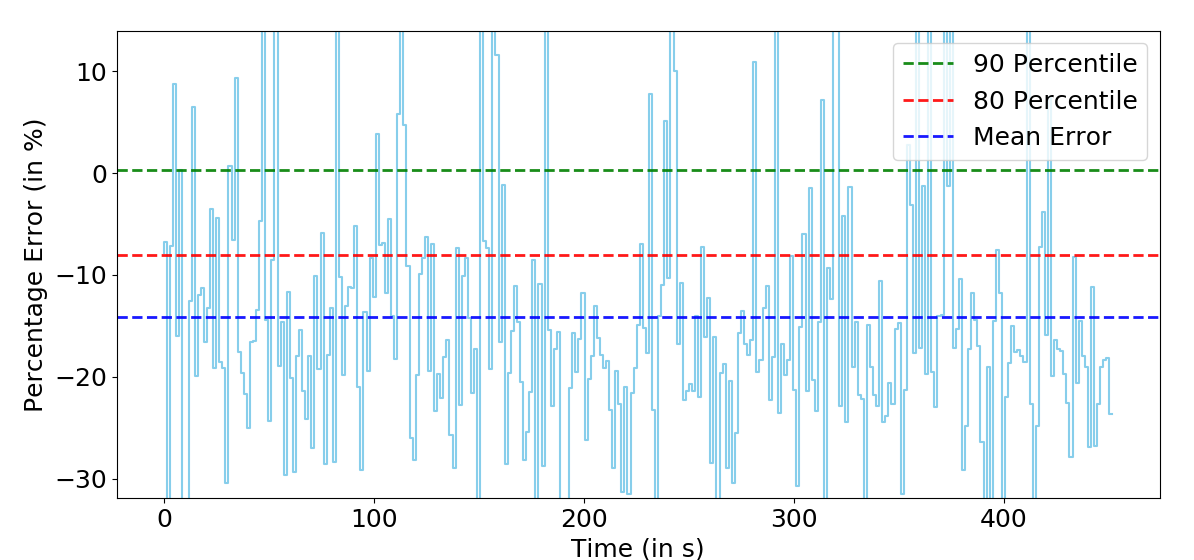
\includegraphics[width=\textwidth]{figures/sensor_error_timeline_5.png}
         \caption{Timeline on Moto Z3}
         \label{fig:sensor_error_timeline}
     \end{subfigure}
     \hfill
\fi

\begin{minipage}{0.48\columnwidth}
\begin{subfigure}[b]{\textwidth}
         \centering
         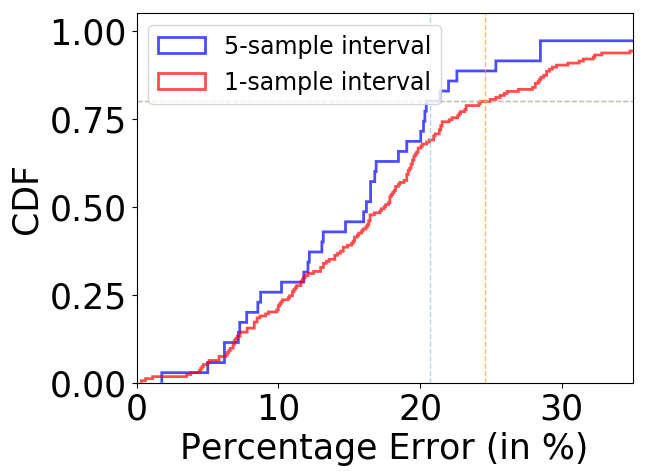
\includegraphics[width=\textwidth]{figures/sensor_error_cdf.png}
         % \caption{CDF for Moto Z3}
%         \label{fig:sensor_error_cdf_motoz3}
     \end{subfigure}
     
  \if 0
  \begin{subfigure}[b]{0.46\columnwidth}
         \centering
         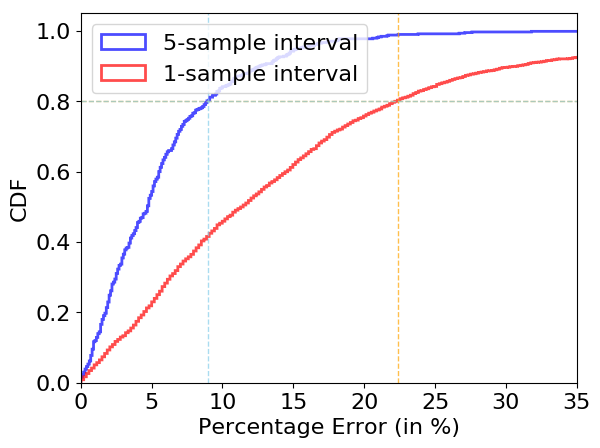
\includegraphics[width=\textwidth]{figures/sensor_error_cdf_nexus6.png}
         \caption{CDF for Nexus 6}
         \label{fig:sensor_error_cdf_nexus6}
     \end{subfigure}
  \fi
  \caption{Power sensor reading error relative to power monitor reading
        for the YouTube for Moto Z3.
        % In CDF, the orange line represents the 80 percentage for 1 sample and blue line represents for 5 sample
        }
        \label{fig:sensor_error}
        \vspace{-0.1in}
\end{minipage}
\hfill
\begin{minipage}{0.48\columnwidth}

    \centering
    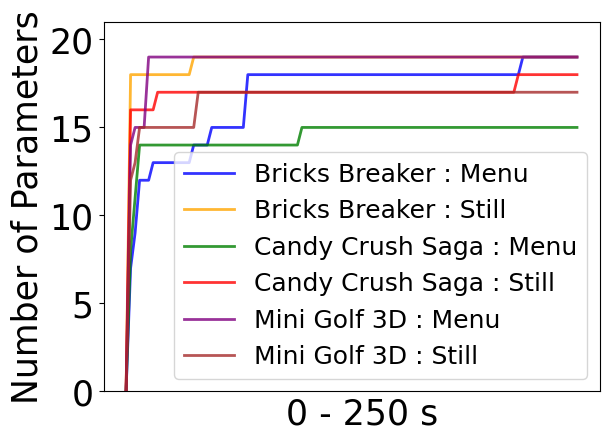
\includegraphics[width=\textwidth]{figures/004_Pixel4_cummulative_macro_parameters.png}
    \vspace{-0.1in}
    \caption{The cumulative number of unique parameters over app run duration on Pixel 4.}
    \label{fig:number_parameters_vs_duration}
    \vspace{-0.1in}
\end{minipage}
\end{figure}


 
To validate the energy counter reading accuracy comparing it with the high-fidelity 
external power monitor readings as the ground truth,
we generated a 250-second run with the YouTube app while the device is connected to the power monitor.
We chose YouTube as it is a popular app and exhibits significant power variations during its run.

%{\bf Findings}
%% 3. Explain power sensor is effects the accuracy of the equations
%Figure~\ref{fig:sensor_error} shows the timeline and the CDF for the sensor error.
\if 0
Figure~\ref{fig:sensor_error_timeline} shows the percentage error of the estimated energy
for 1-sample intervals (1.4s) based on power sensor reading over the 500s app run for Moto Z3.
We observe that \comment{for 89.7\% of the intervals the power sensor reading underestimates the energy drain compared to the power monitor reading.}
\fi

Figure~\ref{fig:sensor_error} shows the CDF for the absolute percentage error on Moto Z3
for 1-sample and for 5-sample intervals (7s). 
We plot the error for 5-sample intervals to see if averaging out over 5 samples can reduce the 
power sensor reading error.
% since if so we can set up an equation for each 5-sample interval as opposed to each 1-sample interval.
However, we see that the average error for 5-sample intervals, 15.84\%,
is only slightly better compared to 1-sample intervals of 19.01\%, and
the 80th percentile errors are 20.52\% and 24.18\% and median errors are 
16.76\% and 17.99\%., respectively.
\if 0
% , and the 80th percentile errors are 24.03\% and 21.10\%, respectively.
% Nexus 6
Figure~\ref{fig:sensor_error_cdf_nexus6} shows the CDF for the absolute percentage error
for 1-sample intervals (175 ms) and for 5-sample intervals (875 ms) for Nexus 6.
However, we see that the average error for 5-sample intervals, 7.21\%,
is lower than for 1-sample intervals of 19.06\%, and
the 80th percentile errors are 9.89\% and 26.60\%, respectively.
\comment{We observe that the sensor is about 3 times lower in Nexus 6 as compared to Moto Z3
for 1 sample interval is due to the interval of Nexus 6 being 8 times shorter than Moto Z3.
Suggesting that the low sampling rate of the sensor is the cause of the error.}
\fi
Such high error suggests that the built-in power sensor readings available on today's Android phones 
are not suitable for self power model derivation. 
Thus we conduct our SPMD verification study by using the external Monsoon power monitor to generate the 
power draw ground truth. 

\if 0
{\bf Reason }
%% 5. Reasons for the inaccuracies in power sensor
The high inaccuracy of the power sensor could be attributed to mainly 2 reasons.
\begin{itemize}
    \item {\bf Noise: } The power management circuit and it's location in the device is susceptible to noise due to the electronic circuitry involved in it.
    It can be argued that, the noise can be reduced by taking a longer interval which might average out the effect of noise, but from our finding we find that this approach is not effective.
    
    \item {\bf Low Sampling rate: } The power sensor generate a new value every 1.4 seconds interval in moto Z3.
    This greatly inhabits use of the power sensor to gather instantaneous current. 
 \end{itemize}
\fi


% The Monsoon power monitor has a sampling rate of 5 KHz  and has been widely used as the ground truth in smartphone power modeling and energy drain studies. 


\subsection{How to Set up Equations?}

The basic SPMD methodology does not specify how to set up systems of equations for the regression solver. Since SPMD is "in-situ", \ie deriving all the power model parameters experienced during a given app run,
in principle we need to create equations those can cover the entire app run duration.
Given an app run of duration $T$, 
we can potentially chop it into $N_s$ equal-sized intervals,
and set up $N_e$ equations per each interval, each covering a duration of $t_e$ of the app run, \ie
\begin{eqnarray}
T = N_s \cdot N_e \cdot t_e
\end{eqnarray}
%
Thus, setting equations for SPMD has two degrees of freedom: 
(1) How many systems of equations $N_w$ shall we create for an app run? 
(2) How many equations $N_e$ shall we create for each interval?
Our verification study explores how the two degrees of freedom can 
help us to improve the diversity for the systems of equations. 


%%%%%%%
\subsection{How to Validate Models from SPMD?}

Since the motivation of SPMD is to capture power model's dependence on app usage, SPMD is fundamentally different compared to learning in TPMD as the goal is not to train a model based on training data from some app run that will predict well the testing data for a different app run. Rather, the goal of SPMD is to generate the power model that best fits a given app run. However, this also raises a fundamental challenge in terms of how to validate the derived model as we generally do not have the ground-truth power model for a given app run. 

{ 
In our verification study, we apply a three-pronged criteria to determine whether the derived SPMD  model is considered acceptable: 
(1) The trend of the model parameters derived should appear similar to the model derived using TPMD. For example, they should be positive, follow monotonicity (\eg CPU power should grow with higher frequency), and the GPU Idle power should be less than the GPU Busy power;
(2) The specific values of the parameters should be within a threshold of their counterparts if compared with the TPMD derived model parameters. The threshold could be based on empirical evidence, \eg from the power state variation study in \S\ref{sec:primer}.
(3) We apply conventional training-testing validation by extracting interleaved training and testing data in a given app run to compare the fitting error for the training and testing data. 
}

%%%%%%%
\subsection{Aligning Power Monitor with Linux event trace}
% \begin{figure*}
%     \centering
%      \begin{subfigure}[b]{0.15\textwidth}
%          \centering
%          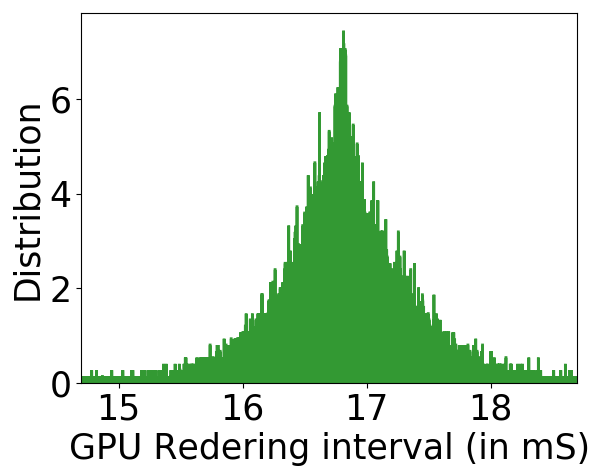
\includegraphics[width=\textwidth]{figures/distribution_interval_bricksbreaker_intro.png}
%          \caption{Bricks Breaker Intro scenario}
%      \end{subfigure}
%           \begin{subfigure}[b]{0.15\textwidth}
%          \centering
%          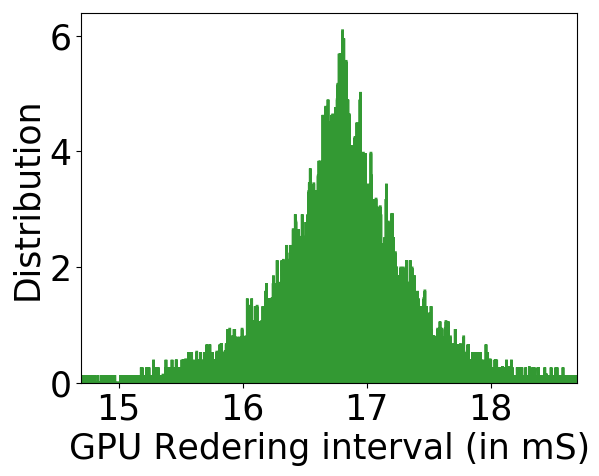
\includegraphics[width=\textwidth]{figures/distribution_interval_bricksbreaker_still.png}
%          \caption{Bricks Breaker Still scenario}
%      \end{subfigure}
%           \begin{subfigure}[b]{0.15\textwidth}
%          \centering
%          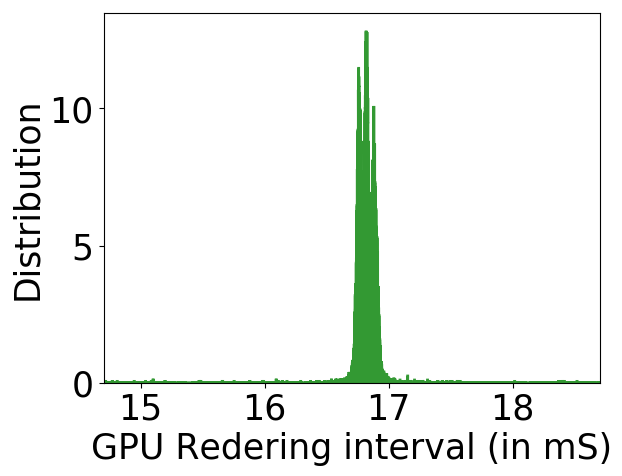
\includegraphics[width=\textwidth]{figures/distribution_interval_candycrush_menu.png}
%          \caption{Candy Crush Menu scenario}
%      \end{subfigure}
%           \begin{subfigure}[b]{0.15\textwidth}
%          \centering
%          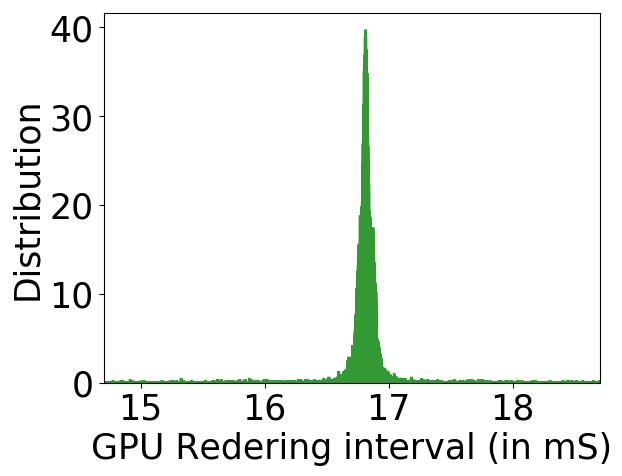
\includegraphics[width=\textwidth]{figures/distribution_interval_candycrush_tutorial.png}
%          \caption{Candy Crush Tutorial scenario}
%      \end{subfigure}
%           \begin{subfigure}[b]{0.15\textwidth}
%          \centering
%          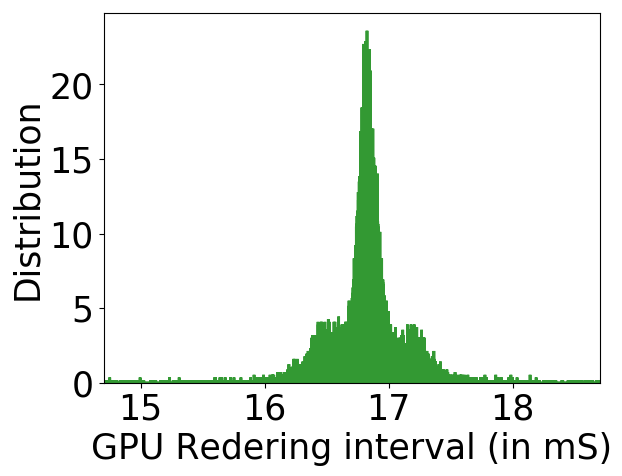
\includegraphics[width=\textwidth]{figures/distribution_interval_pottery_intro.png}
%          \caption{Pottery Intro scenario}
%      \end{subfigure}
%           \begin{subfigure}[b]{0.15\textwidth}
%          \centering
%          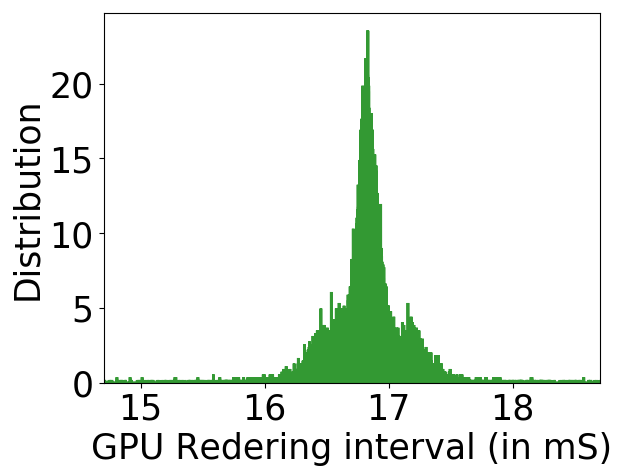
\includegraphics[width=\textwidth]{figures/distribution_interval_pottery_create.png}
%          \caption{Pottery Create scenario}
%      \end{subfigure}
%      \caption{Distribution for GPU redering interval}
%     \label{fig:distribution_gpu_interval}
% \end{figure*}
A modern smartphone on an average can generate 60 frame per second. 
From the event trace we found that the time taken to generate frames by the GPU can vary.
% Figure~\ref{fig:distribution_gpu_interval} shows the rendering interval spread
% for the 6 app scenarios collected from event trace.
The standard deviation to generate frames is found to be in  the range of 0.37 to 1.51 ms.
Figure~\ref{fig:power_trace_candycrushturorial} shows a typical rendering interval.
We first mark the rising edge on the power monitor trace as the start of the interval and 
the fall edge as the end of the GPU Active-busy state.
We choose a 50 interval window from the middle of the power monitor trace which has lowest standard deviation
for both the total rendering interval as well as GPU Active busy duration.
Then, from the event trace we use a sliding window to find out the window 
which scales best to those 50 windows of the power monitor  .
\comment{Further, for micro and nano analysis, on a per rendering interval basis,
we scale the rendering interval duration from power monitor trace to match that of the rendering
duration of the event trace interval per interval basis.}
% We choose a 50 interval window which we slide across 10 seconds in the middle of the trace.
% The cost function chosen is the L1-norm of the standard deviation of the total interval and
% the GPU Active-busy interval. We choose the 50 interval which has the least standard deviation.
% To align it with the event trace, we use L2 norm of the difference in the total interval
% and GPU Active-busy interval over a sliding window. 